The main study was designed to validate the results of the pilot study over different locations at different times. 
We choose five different locations across central London, to install the sensors and collect data for a long period of time. 
We also carry out manual counting on these locations along with this across different time of the day. 
We then apply the filtering based on signal strength and sequence numbers and compare with manual counts and evaluate the effectiveness of the process with the mean error per minute on these locations. 
Finally we calculate the ajustment factor for the first interval of manual counts and check if that works on the consecutive intervals. 

The locations where the data were collected are shown in the table. The location are chosen for their variety of configuration and sources of noise. Location 1 is the `cleanest' of while location 2 is the one with the most complexity. The configuration, installation and data collection schedule is shown in the figure. 

\begin{table}
	\tbl{Locations where sensors were installed}
	{\begin{tabular}{clll} 
		\toprule
		 ID & Location & Type & Installation notes\\
		 \midrule
		 1 & Camden High Street & Phone Shop & Bus stop in front\\
		 2 & Central St.Giles Piazza & Restaurant & Seating area on both sides\\
		 3 & Holborn Underground Station & Information Kiosk & Overlooks station entrance\\
		 4 & Brunswick Center & Fast Food Restaurant & Has seating area on one side\\
		 5 & The Strand & Tea Shop & Has phone shop next door \\
		 \bottomrule
	\end{tabular}}
	\label{locations-table}
\end{table}

\begin{figure}
	\begin{center}
		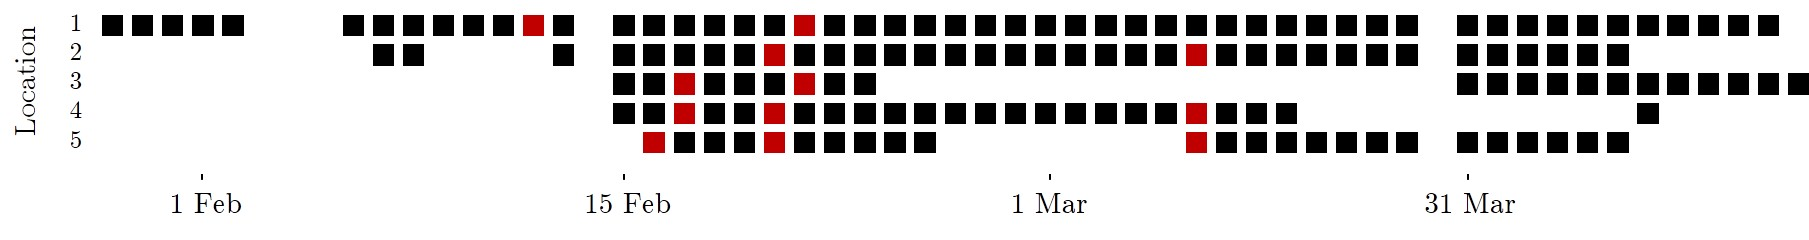
\includegraphics [width=0.90\linewidth] {images/main_schedule.jpeg}
		\caption{Days when the sensors were active at the corresponding location. The red square shows that manual data collection was also done.}
		\label{pilot_clustering}
	\end{center}
\end{figure}

Though data was collected for many continous days, for the purposes of comparing with ground truth we just consider the only the data from sensors corresponding to those sessions. We have 12 sets of data over 6 different days. We have atleast two set manual counts for each location for verification of calibration.

\subsection{signal strength filtering}
First we see the distribution of the signal strength varies with location and configuration. 
The density plot for signal strength is shown alogn with configuration in figure.
We can see that the signal strength distribution shows distinct patterns of high and low when the installation is that there is a clear distant source of noise but this distinction get more and more obscure as we move towards difficult installations. 
For example, location 2 is almost a normally distributed noise as it is too far to pick up any pedestrians but location 5 with a clear view of footpath and a phone shop next door shows clear distinction between the two. 
Intuitively the classfication algorithm should give us better results in the latter. 
It is important to note that we are dealing with relative singal strengths, this can vary with location and time of the analysis but we should be still be able to differentiate signal from noise. 
We run the kmeans classification algorithm and filter out the probe requests which are randomised and have signal strengths less than the second break (or the threshold). 
We then count the number of Unique MAC addresses present in every minute and remove MAC addreses which reappear within 30 minutes of previous appearance. 
We then compare this with the minute by minute aggreagation for the manual counts and find the average error per minute for the sensor count. 
The results are shown in the table.We see that the location XXXX has the most error while location XXX has the least error confirming our intuition. 
We also see that the error follows the complexity of the installation. 
It is also very promising that this method alone reduces our margin of error by a lot. 
For some practical purposes which does not require absolute numbers, this should be sufficient. talk about examples of indexes and dashboards and short term trends. 

\begin{figure}
	\centering
	\subfigure[Installation configuration of sensors at various locations]{
		\resizebox*{0.46\linewidth}{!}{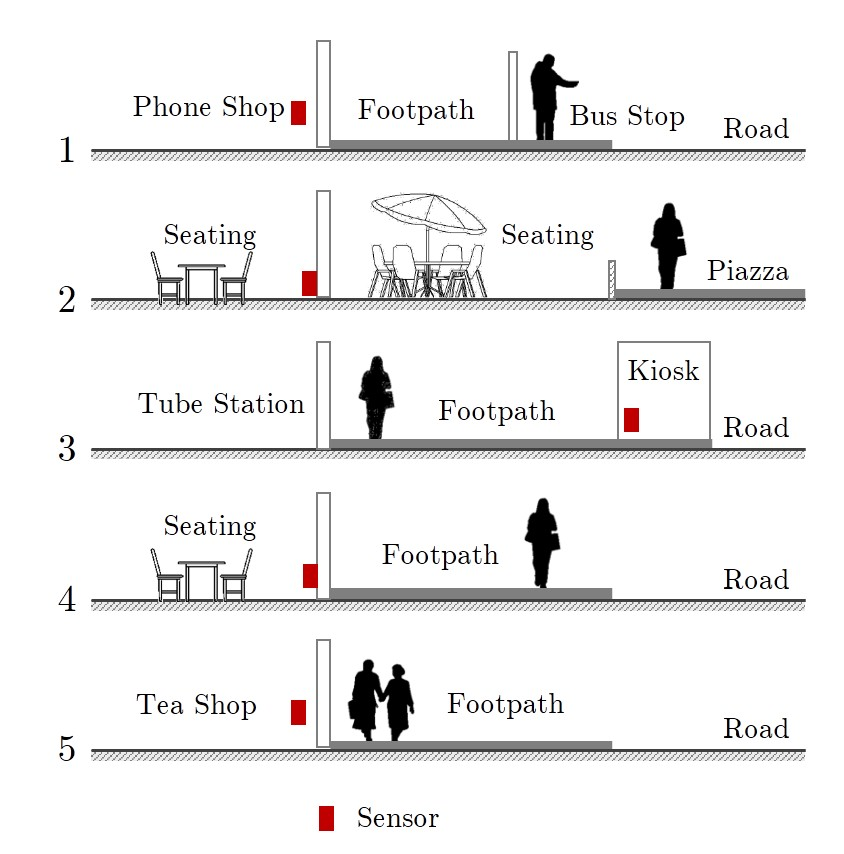
\includegraphics[trim=20 6 20 6,clip]{images/main_configs.jpeg}}}\hspace{20pt}
	\subfigure[Density distribution of signal strength (lower values show higher signal strength)]{
		\resizebox*{0.46\linewidth}{!}{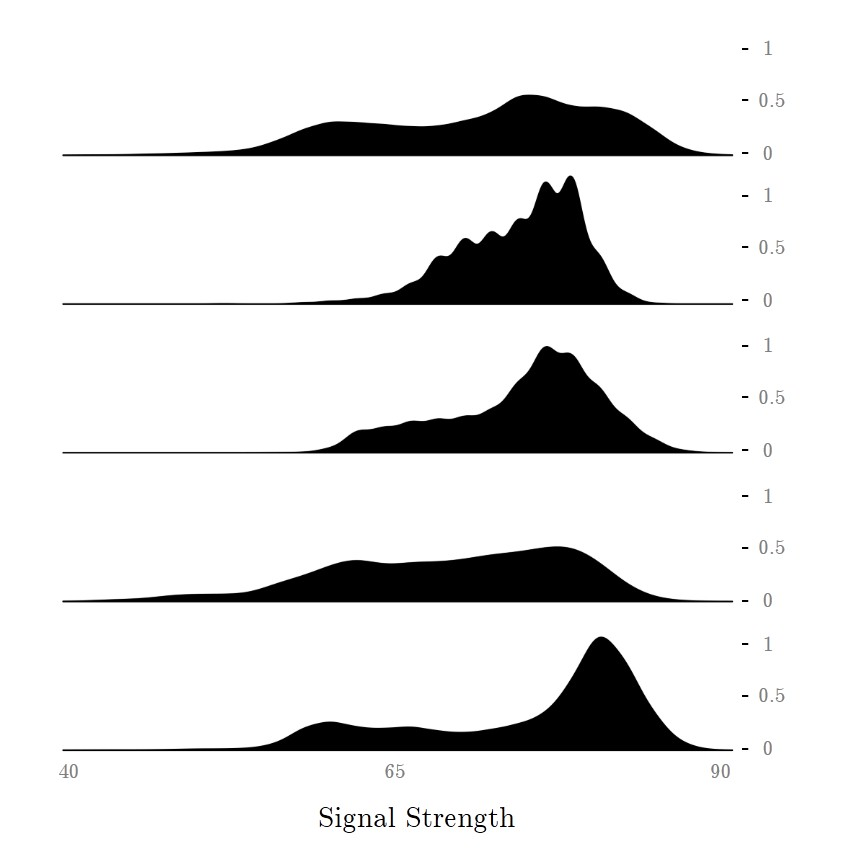
\includegraphics[trim=20 4 25 6,clip]{images/main_signals.jpeg}}}
	\caption{Distribution of signal strengths across locations} \label{methodology_schematic}
\end{figure}


The comparision between global and local.
comparision between different types of vendors.
Specifics on top 5 manufacturers.

This is also done for different locations hourly for all the data we had.
we compare it to the manual counts and see that the average mean error
has been reduced/increased. The finger print works well for all the locations.
It also works over a period of time and gives us a comparable and close 
footfall count to the manual count. The thresholds found in the pilot study
works as well.

Finally we normalise the sensor counts to match the manual count using
a fraction/ adjustment factor calculated from the know manual counts.
we have three sets of counts. We check if the adjustment factor holds the
same in all three counts across locations. It does with a variations from
xxx to xxx. The results are shown in the table. 

we see that the signal strength filtering works and reduces error by
xxxxx. there is variation by locations.
we see that sequence number algorithm works as well. The threshold stays
constant well and works well across locations. The calibration also works
and ajustment factor stays consistent short term. This needs more work 
long term.
